\documentclass[a4paper,11pt]{amsart}
\usepackage{amssymb}
\usepackage[T1]{fontenc}
\usepackage{indentfirst}
\usepackage{enumerate}
\usepackage{stmaryrd}
\usepackage{xspace}
\usepackage{amsmath}
\usepackage{amsfonts}
\usepackage{url}
\usepackage[colorlinks=true, a4paper=true, pdfstartview=FitV,
linkcolor=blue, citecolor=blue, urlcolor=blue]{hyperref}
\pdfcompresslevel=9

\usepackage[left=2.61cm,right=2.61cm,top=2.72cm,bottom=2.72cm]{geometry}


\usepackage{graphicx}
%%%%%%%for quotes
\usepackage{textcmds}

\usepackage[english,frenchb]{babel}
%\usepackage[latin1]{inputenc}
\usepackage[utf8]{inputenc}
\usepackage{indentfirst, amsfonts, amsmath, amsthm, amssymb, amscd}
\usepackage{amsmath,amsfonts,amscd,bezier}
%%%%%%%%%%%%%%%%%%%%%%%%%
\usepackage[most]{tcolorbox}
%%%%%symbol for EUR
\usepackage{eurosym}
%%%%%%%%
\begin{document}
\begin{tcolorbox}[center,colback=white]
\begin{center}
{\large\textsc{Lending Club: Borrowing and Investing Money}}\\
\end{center}
\end{tcolorbox}

\vspace{.1cm}

\section{Description}
The idea of lending money for profit has long been around. As a result, many successful companies have built their business strategy based on lending money to businesses or private individuals. 

\medbreak

The way we borrow money and the way we invest money have changed. Back in the day, if you wanted a loan to pay off your car or credit cards, you’d go to a bank or a credit union, sit down with a loan officer, and wait for them to tell you yes or no as they “crunched the numbers.” Investing was always done with a traditional broker—online or in-person. Nowadays, people use techniques from Data Science and Machine Learning to validate models and so, it makes life easier for potential customers, as they will be directed on how they should invest their money. As a simple result, companies can analyse a credit risk scenario, and so the loss is minimum and the profit is maximized. 

\medbreak

In this project, we will use loan data from Lending Club, a US peer-to-peer lending company. Borrowers on the platform can borrow between $\$1,000$ to $\$40,000$ in the form of unsecured personal loans, for a term of either three or five years.

\medbreak

Investors can browse the loan applications and choose to finance the loans based on the credit history of the borrower, the amount of the loan, the loan grade, and the purpose of the loan. Investors earn money through interest paid on the loans, and Lending Club makes money from loan origination fees and service charges.

\medbreak 

The loan dataset used in this work is from $2007$ to $2011$ and is available at the \href{https://www.lendingclub.com}{Lending Club Website}. Throughout this project, we use Python libraries for the analysis of our dataset as well as for training the machine learning models. More precisely, we use Pandas library to import the dataset, prepare/clean it, and identify the features and the target. For visualizing the dataset we use Searborn library and finally to train machine learning algorithms we use Scikit learn library. Many of code reproduced herein are adapted from 

\begin{flushleft}
Ankur A. Patel, \textit{Hands-On Unsupervised Learning Using Python: How to Build Applied Machine Learning Solutions from Unlabeled Data}, Oreilly Media, 2019.
\end{flushleft}

\medbreak

Now, let us briefly explain how we plan to present our analysis and results. In the first stage, we employ exploratory data analysis to do the data cleaning. We identify these fields include attributes of the loan and attributes of the borrower. Then, we proceed to study these fields in more details by transforming strings format to numerical format, and imputing missing values. Our plan is to employ clustering analysis to get our results. Since it is an unsupervised learning approach, labels are not used. However, to judge the goodness of our clustering algorithm at finding distinct and homogeneous groups of borrowers in this Lending Club dataset, we will use the loan grade as a proxy label.

\medbreak

In order to evaluate the goodness of the clusters, we create an $X$-train matrix with all of our $34$ numerical features, and a $y$-train with the numerical loan grades, which we use only to validate the results, \textbf{not} to train with the algorithm. First, we employ \emph{k-means} clustering, and to get the best value for the desired clusters $k$ we use the elbow method and analyze the best performing k measure. Next, we employ \emph{Hierarchical Clustering}, which we do not need to set to a particular number of clusters. To do that, we use \emph{fastcluster}. Then, we employ \emph{HDBSCAN, MiniBatchKMeans, Agglomerative Clustering, OPTICS}, and \emph{MeanShift}.

\medbreak

In Section \ref{problem}, we present the formal problem and mention our target audience. In Section \ref{dataanalysis}, we explain the data cleaning, data visualization, and the unsupervised methods used in this project. In Section \ref{results}, we present the key findings of our analysis and discuss the results obtained. Finally, in Section {future}, we discuss about the accuracy of each method, and possible ways to improve them.

\medbreak

Last but not least, we mention that in order to clarify our analysis, and give a clear presentation of the results therein obtained, we add the notebook file to this report. 

\section{Problem Statement \& Target Audience}\label{problem} 

Our goal is to perform group segmentation on the loan dataset, i.e., identify the underlying structure and group clients based on similarity. We plan to separate groups according to their characteristics, and so we can predict higher return on investment and lower loss on loan. 

\medbreak

The techniques and methods used in this project illustrate how we can approach an unsupervised learning problem of clustering type. Although we use the loan dataset from Leading Club, we can easily adapt our approach to deal with similar problems. Our target is any lending company, and clients who wish to borrow money and obtain highest return on investment.

\section{Data Analysis}\label{dataanalysis}

We begin our analysis by getting the dataset, which is available at \href{https://www.lendingclub.com/}{Lending Club}. It contains data on loan in the company from $2007$ to $2011$. 
\medbreak

The number of instances (rows) in the data set is $36,022$, and the number of variables (columns) is $145$, but most of these columns are empty and are of little value to us. Therefore, we will designate a subset of the columns that are mostly populated and are worth using in our clustering application. These fields include attributes of the loan such as the amount requested, the amount funded, the term, the interest rate, the loan grade, etc., and attributes of the borrower such as employment length, home ownership status, annual income, address, and purpose for borrowing money. In this new subset of features, our data has $36,022$ loans and $37$ features. So, we reduce from $145$ to $37$ relevant columns!

\medbreak

Next, we deal with the data engineering. First, we transform string format to numerical format in a certain subset of columns. For our clustering application, we will consider just the numerical features and ignore all the categorical features because nonnumerical features cannot be handled by our clustering algorithms in their current form. To do that, we use a \emph{lambda} function. Then, we proceed to impute missing values. We find these numerical features and count the number of NaNs per feature. We will then impute these NaNs with either the mean of the feature or, in some cases, just the number zero, depending on what the feature represents from a business perspective. To do that, we use \emph{Imputer} method from \texttt{sklearn.preprocessing} together with a \emph{lambda} function. 

\medbreak

Next, we select final set of features and perform scaling. We will generate the training dataframe and scale the features for our clustering algorithms. To judge the goodness of our clustering algorithm at finding distinct and homogeneous groups of borrowers in this Lending Club dataset, we will use the \emph{loan grade} as a proxy label. The \emph{loan grade} is currently graded by letters, with loan grade "A" as the most credit-worthy and safe and loan grade "G" as the least. There are some NaNs in the loan grade. We will fill these with a value of "Z" and then use the LabelEncoder from Scikit-Learn to transform the letter grades to numerical grades. To remain consistent, we will load these labels into a "$y$-train" Python series. We then compare loan grades with interest rates. 

\medbreak

Finally, we define a function to evaluate how good our models predict the segmentation of the borrowers into clusters. If the clustering algorithm does a good job separating the borrowers in the Lending Club dataset, each cluster should have borrowers that are very similar to each other and dissimilar to those in other groups. Presumably, borrowers that are similar to each other and grouped together should have similar credit profiles -- in other words, their creditworthiness should be similar.

\begin{figure}
 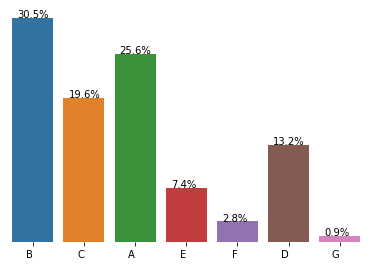
\includegraphics[width=.5\linewidth]{download.png}
  \caption{Loan Grades}
  \label{fig:loan}
\end{figure}

\medbreak

\noindent{\textsc{k-Means}.} Recall that we need to specify the desired clusters $k$, and the algorithm will assign each borrower to exactly one of these $k$ clusters. Instead of specifying just one value of $k$, we will run an experiment where we set k from a range of $10$ to $30$ and plot the results of the accuracy measure we defined in the previous section. We obtain that the accuracy is best around $30$ clusters.

\medbreak

\noindent{\textsc{Hierarchical Clustering}.} Recall that in hierarchical clustering we do not need to set to a particular number of clusters. Instead, we can choose how many clusters we would like after the hierarchical clustering has finished running. Using \emph{fcluster} we find that the number of distinct clusters is $25$.

\medbreak

\noindent{\textsc{HDBSCAN}.} Recall that \emph{HDBSCAN} will group borrowers together based on how closely packed together their attributes are in a high-dimensional space. Unlike \emph{k-means} or \emph{hierarchical clustering}, not all the borrowers will be grouped. Some borrowers that are very distinct from other groups of borrowers may remain ungrouped. These are outlier borrowers and are worth investigating to see if there is a good business reason they are dissimilar from other borrowers. We find that the number of distinct clusters is $9$.

\medbreak

\noindent{\textsc{MiniBatchKMeans}.} Recall that in comparison with \emph{k-means}, the MiniBatchKMeans is faster, but gives slightly different results. We use 30 clusters to separate the borrowers and then we compare their overall accuracies.

\medbreak

\noindent{\textsc{Agglomerative Clustering}.} This method recursively merges the pair of clusters that minimally increases a given linkage distance. We set the clusters to be $30$ and compare their overall accuracies.

\medbreak

\noindent{\textsc{OPTICS}.} This method is closely related to DBSCAN, and finds core sample of high density and expands clusters from them. Unlike DBSCAN, keeps cluster hierarchy for a variable neighborhood radius. It's in general best suited for large datasets. Nevertheless, we played around with it and obtain that the number of clusters is $136$! So, we will not take its accuracy to get insight from the dataset.

\medbreak

\noindent{\textsc{Mean Shift}.} We use \emph{estimate bandwith} from \texttt{skelarn.cluster} to get the value for the bandwith term. The number of estimated clusters is $27$.

\section{Key Findings}\label{results}

In this section, we discuss the accuracy results obtained in this project. Let us begin with the k-means algorithm. 

\medbreak

The accuracy of \emph{k-means} varies quite a bit from cluster to cluster. Some clusters are much more homogeneous than others. For example, on cluster has an accuracy of $73.41\%$, while cluster other has an accuracy of just $22.99\%$. This is a starting point to build a clustering application to automatically assign new borrowers that apply for a Lending Club loan into a preexisting group based on how similar they are to other borrowers. Based on this clustering, it is possible to automatically assign a tentative numerical loan grade to the new borrower, which will be correct approximately $41.31\%$ of the time. Next, we give the overall accuracy for each clustering method.
\begin{table}[h!]
  \begin{center}
    \caption{\textsc{Clustering}}
    \label{tab:table1}
    \begin{tabular}{l|c|c|} 
      \textsc{Algorithm}& \textsc{Number of Clusters} &\textsc{Overall Accuracy}\\
      \hline
       \textsc{k-Means}& 30  &41.31\%\\
       \hline
        \textsc{Hierarchical}& 25  &38.94\%\\
       \hline
        \textsc{HDBSCAN}& 9 &31.20\%\\
       \hline
        \textsc{MiniBatchKMeans}& 30  &40.82\%\\
       \hline
        \textsc{Agglomerative}& 30  &40.14\%\\
       \hline
        \textsc{OPTICS}& 136  &30.52\%\\
        \hline
         \textsc{MeanShift}& 27  &30.74\%\\
       \hline
    \end{tabular}
  \end{center}
\end{table}

\medbreak

The Hierarchical overall accuracy is  $38.94\%$, which is a bit worse than with k-means clustering. That being said, hierarchical clustering works differently than k- means and may group some borrowers more accurately than k-means, while k- means may group other borrowers more accurately than hierarchical clustering. In other words, the two clustering algorithms may complement each other, and this is worth exploring by ensembling the two and assessing the ensemble’s results compared to the results of either standalone solution. As with k-means, the accuracy varies quite a bit across the clusters. Some clusters are much more homogeneous than others.

\medbreak

The HDBSCAN overall accuracy is $31.20\%$, which is much lower than in the previous two algorithms. Among the accuracy by cluster, the accuracy ranges from $29\%$ to $100\%$, but has a poor accuracy if we plan to segment a given borrower into one of the clusters.

\medbreak

The MiniBatchKmeans and Agglomerative clustering algorithms give similar overall accuracies. As we have previously mentioned, the results of the OPTICS algorithm shouldn't be taken into account, since it is best suitable for large datasets. We have obtained a segmentation into 136 clusters! Finally, MeanShift gives comparable number of clusters, but fails to give a better overall accuracy.

\begin{figure}
 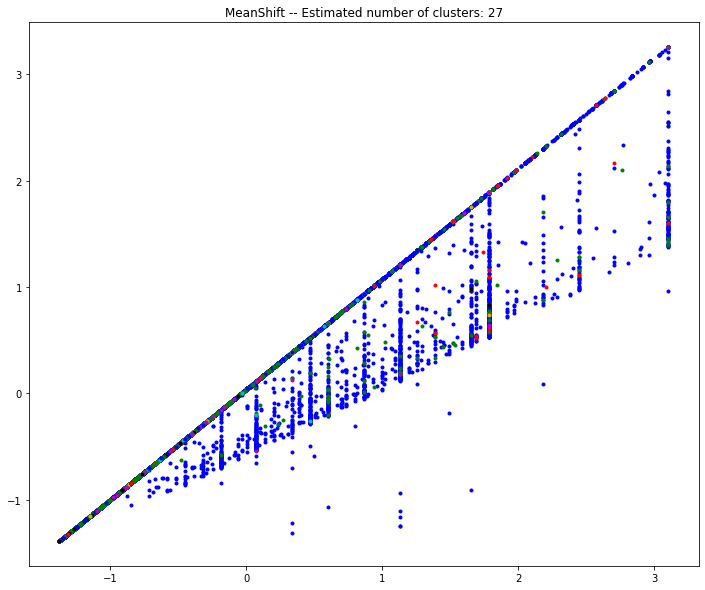
\includegraphics[width=.8\linewidth]{download-1.png}
  \caption{MeanShift with 27 clusters}
  \label{fig:loan}
\end{figure}

\section{Final Comments}\label{future}
In this project, we built an unsupervised clustering application based on borrowers that applied for unsecured personal loans on Lending Club from $2007$ to $2011$. The applications were based on k-means, hierarchical clustering, hierarchical DBSCAN, MiniBatchKmeans, Agglomerative, OPTICS and MeanShift, with k-means having the best performance, scoring an approximately 4$1\%$ overall accuracy.
While these applications performed okay, we believe they can be improved quite a bit. 

\medbreak

We should consider whether acquiring more data, performing more feature engineering and selection, selecting different parameters for the k-means algorithm, or changing to a different clustering algorithm will improve the results. It is possible that we do not have enough data to meaningfully separate the borrowers into distinct and homogeneous groups more than we have already; if this is the case, more data and more feature engineering and selection are required. Recall also that we only used a subset of columns and performed our studies therein. It's possible that we may have neglected some useful information. Besides there were many NaN values. 

\medbreak

Finally, let us mention that a good starting point for a future project would be an implementation of Deep Learning techniques, e.g., using TensorFlow and Keras libraries.
\end{document}